% appendices.tex

\section{Appendices}

% Not yet ready for prime time; may not include it at any rate because
% of the "negative-zero" problem.

\subsection*{Higher Order Exponents}

You can multiply a number times itself as many times as you want. Understanding a little more about exponents (the number of times you multiply a number times itself) will make understanding the language we use to discuss computers quite a bit easier. Just as we mention kilobytes and megabytes as units of storage, there are also less common units of storage that invent new multiplier terms for bits and bytes, because of the ``powers of 2.'' So let's learn about base-2 exponents-- the ``powers of two".

\bigskip
\newcommand{\expline}[2]{
$2^{#1}$ & = & #2 
}

\begin{footnotesize}
\begin{tabular}{l c l p{3.5in} }

\multicolumn{3}{c}{\textbf{Powers of Two}} & \textbf{Notes} \\ 
\hline\\[\negsep]

\expline{0}{1}& This one is strange, sort of. But it works! Any number ``to the zeroth power" is equal to 1. See below for more. \\
\expline{1}{2} \\
\expline{2}{4} \\
\expline{3}{8} \\
\expline{4}{16} & Since $2^2 = 4$, $2^2 \times 2^2 = 16 $   \\
\expline{5}{32} &  This is why you can count to 31 on one hand. \\
\expline{6}{64} \\
\expline{7}{128} \\
\expline{8}{256} & 8-bit computers were the first machines really adopted by consumers. Also, 8 bits makes up one \emph{byte} of computer memory, so each byte can take on up to 256 values. \\ 
\expline{9}{512} \\
\expline{10}{1,024} & 1,000 usually gets the prefix \emph{kilo-}, like a kilogram is 1000 grams. A \emph{kilobyte} is 1024 bytes.\\
\expline{16}{65,536} \\
\expline{20}{1,048,576} & $2^{10}$ bytes is a kilobyte; ($2^{10} \times 2^{10}$) bytes is a \emph{megabyte}.\\
\expline{24}{16,777,216} & Most computer displays can show up to 16 million colors, using red, green, and blue, all in combination. Each piece of the color can have 256 ($2^8$) levels, from zero (black) to 255 (100\% red, or green, or blue)\\
\expline{30}{1,073,741,824} & $2^{30}$ bytes is a \emph{gibibyte}, or a bit more than a \emph{gigabyte}, which is 1000 megabytes. \\
\expline{32}{4,294,967,296} \\ 
\expline{40}{1,099,511,627,776} & $2^{40}$ bytes is a \emph{tebibyte}, or a few percent more than 1000 gigabytes -- a \emph{terabyte.} \\
\expline{50}{1,125,899,906,842,624} & $2^{50}$ bytes is \emph{pebibyte}. A petabyte is so large that one pebibyte is enough to store the DNA of the entire population of the USA\ldots{}and then clone them, \emph{twice.} \\[\sep]
\hline
\end{tabular}

\end{footnotesize}
% $10^2 & = & 100 & \\
%$10^3 & = & 1000 & \\
%$10^4 & = & 10000 & \\

\vfill

\stbox{6.0in}{\emph{Explanation:} The reason that any number to the zeroth power is equal to one comes from the way we subtract exponents when dividing. You know that 8 divided by 4 equals 2; written another way, $2^3 \div 2^2 = 2^1$. Notice that the exponents change by subtraction, but the equation is the same! You can \emph{divide} base-exponent numbers by \emph{subtracting} the exponents (\emph{extra-special historical trivia: this is how slide rules work}; see Figure \ref{fig:sliderule} for a picture). And since any number divided by itself equals one, as in $2^3 \div 2^3 = 1 $, subtracting the exponents gives $2^0$.}


%\subsection*{Negative Numbers}
%
% If we had told the computer that it was using \emph{signed} numbers, it would count upwards from -32,768, and the first column would be a one, to indicate it was negative, with the rest of them zeros. That is, the format for storing negative numbers subtracts 32,768 from 0 -- the range is still the same (65,536 numbers), but the starting point is different. 

\subsection*{Numbers Below Zero?}

Representing \emph{positive} numbers is easy for a computer: it counts upwards from zero. Representing \emph{negative} numbers is harder, because \emph{taking away values by adding them} is a little awkward. To represent a negative, designers use the leading (left-most) bit to declare ``positive'' (zero) or ``negative'' (one). Note that the \emph{range} of numbers that can be represented does not change -- for a 4-digit binary number, whether counting from zero to 15, or from -8 to 7, the total space used on the number line is still 16 numbers, in order.

\stbox{6.0in}{
\emph{Problem:} If the computer doesn't know it is supposed to use that first number to determine whether a number is negative or not, how does it evaluate the number?
}

\subsection*{Complement of a Number}

In mathematics, the \emph{complement} of a binary number is ``the value obtained by inverting all the bits in the binary representation of the number (swapping 0s for 1s and vice versa)." This number is called the \emph{ones' complement} of the number.\footnote{{\color{webblue}\href{https://en.wikipedia.org/wiki/Ones\%27_complement}{Wikipedia page on Ones' Complement.}}}


Here's an example:

\bigskip

\begin{tabular} {c c c}
 Number &  $+$   &   $-$ \\[\sep]
 \hline\\[\negsep]
 0  &  0000 &  1111  \\ 
 1  & 0001  & 1110  \\
 2  & 0010  & 1101\\
 3  & 0011  & 1100\\
 4  & 0100  & 1011\\
 5  & 0101  & 1010\\
 6  & 0110  & 1001\\
 7  & 0111  & 1000\\
 \hline

\end{tabular}

\subsection*{Subtraction}

Subtraction is similar to addition -- very similar, since the process is ``adding a negative number". To this point, we haven't seen negative numbers, because numbers below zero are harder to create or see, compared to numbers between zero and 15, or some other positive number. To get a negative number, computer scientists decided to create a pattern for describing negative numbers, that computers can correctly interpret. They decided to use the first bit (1 or 0, just a ``yes'' or ``no'' indicator) of the number as the \emph{sign bit}: that is, if the first bit, in a ``signed integer", is 1, then the number is a negative number. So if we have a four bit number, and the first bit is only for the ``is this number negative'' indicator, the number represents numbers in the range $[-7,8]$ -- still 16 values, but counting from $-7$ instead of zero. Also note that if you don't tell the computer the number is signed, it will happily assume the number is \emph{unsigned} and give you the wrong answer\footnote{Well, really, it will give you the \emph{right} answer to a question that is different from the question you thought you were asking!}.

To subtract, we first create the \emph{two's complement} of the number we are subtracting (the ``subtrahend"). We leave the number from which we are subtracting (the ``minuend") alone.

Two's complement works like this: you take the \emph{complement} of the number, and add one. \emph{Complement} means you swap all the zeroes for ones, and all the ones for zeroes. Put another way, you run each bit through a NOT gate, then add a one to the result, using a set of full adders.

Let's take the two's complement of 7.

\begin{verbatim}
       0111      7

       1000           ones' complement of 7
       0001           add one to get two's complement of 7
===========   ====
       1001     -8 + 1 = -7 

\end{verbatim}

So here's a simple example of subtraction:

\begin{verbatim}
       0110      6
-      0011      3
===========   ====

       1100           ones' complement of 3
       0001           add one to get two's complement
===========	   
       1101           (-8 + 1 + 0 + 4) = -3 ... good. Now we can add:


       0110      6
+      1101     -3
===========   ====
       0011      3      (see how the sign bit was converted to positive?)
                        (the overflowed bit doesn't matter in this case)

\end{verbatim}

\newpage
And here's a slightly more interesting one, with 8 bit numbers:

\begin{verbatim}
  0000 0110      6
- 0001 0011     19
===========   ====

  0001 0011     19
  
  1110 1100             ones' complement
  0000 0001             add one
===========   ====
  1110 1101     (-128 + 64 + 32 + 0 + 8 + 4 + 0 + 1) = -19


  0000 0110      6
+ 1110 1101    -19
===========   ====
  1111 0011    -13   (-128 + 64 + 32 + 16 + 0 + 0 + 2 + 1) = BOOM! 
  
\end{verbatim}

\newpage
\section*{A Bit More About Capacitors}

The Leyden jar was one of the first capacitors invented: metal foil was placed inside a glass jar, and wrapped around the outside of a glass jar, but neither foil gets near the top of the jar. The glass barrier between the foil sheets (inside and outside) allows a charge to build up between the foil without allowing the electrical charge to move through the glass. Leyden jars didn't hold much charge, but the concept it demonstrated has not changed.

Capacitors are usually made with two metal plates that are on top of each other (or wrapped around each other), but that do not actually touch. When powered, they allow energy to be stored inside an electrical field. Because the plates need a lot of area to store even a small amount of charge, the plates are usually rolled up into some other shape, such as a cylinder. Sometimes, other shapes of capacitors are used for special purposes. 

\bigskip
\stbox{6.0in}{
\emph{Experiment:} make a variable capacitor from aluminum foil, paper, and a paper towel tube. The paper should go around the roll only once. Cut the foil one-quarter or one-half inch smaller than the paper on all sides. Tape a small wire to one corner of the foil, if possible using metallic/conductive tape\footnote{See below for guidance on soldering to aluminum foil}. Tape the foil to the paper. Tape one edge of the paper, foil side down, against the cardboard tube. Make another paper/foil combination. Wrap the paper/foil around the cardboard tube, but tape the paper only to itself, and just loose enough to slide a little. 

\bigskip

It is also possible to make a regular capacitor with the paper-foil layers, separated by flat sheets of cardboard. Keep track of the ``up'' and ``down'' sides! Note that it is pretty easy to gang each ``plate'' together and make capacitor with a larger value; tying all the anodes together, and all the cathodes together, makes a larger capacitor.
}



\section*{Soldering To Aluminum Foil}

It is possible but not recommended to solder a copper wire to the aluminum foil. Soldering it is pretty hard and also the resulting joint is not very strong. If you want to try it, you'll need to put a big drop of heavy oil (motor oil or soybean oil, say) on the aluminum foil to get anything to solder to a copper wire. The heat from the soldering iron rapidly changes the aluminum into \emph{aluminum oxide} and you cannot solder to aluminum oxide. The oil prevents oxygen from getting to the aluminum (and therefore, the important part of the solder joint), but it's not a very good solution to the problem. The oil will smoke. You should solder outside away from things that burn.

\newpage


%---------------------------
\newpage
\section*{Memory}
%---------------------------

Logic circuits need to store the numbers they are working with in order to do more than one thing. Central Processing Units (CPUs), Arithmetic Logic Units (ALUs) or Floating-Point Units (FPUs) each work with numbers, and need to fetch them from somewhere and put them somewhere when they are done. The ``somewhere" is \emph{memory}. Keeping with the use of binary math and binary logic, a high voltage would be a 1 and a low voltage would be a 0. Through the use of these little stored charges, computers can keep track of many, many pieces of information. No matter what the circuits are doing, everything being stored is composed of some count of zeros and ones. 

There have been \emph{many} forms of memory through the years, including punched paper cards, and even a wiggly wire! The most common memory these days is a circuit made up of six transistors, or one transistor and a capacitor or two. Computers read eight, sixteen, 32, or 64 bits at a time from a row of memory and pass the number, or the instructions, from memory on to be processed.

One type of computer memory, called \emph{static RAM}, uses six transistors per bit instead of one transistor and a capacitor for bit (as used in dynamic ram, the main memory for the computer), so it's bulky, but it's also faster. To store one bit with 6 transistors is also expensive so SRAM is mostly used for very important memory, like the memory very close to the core of the computer processor. Have a look at Figure \ref{fig:sram}\footnote{Diagram and supporting information adapted from {\color{webblue}\href{https://en.wikipedia.org/wiki/Static_random-access_memory}{Wikipedia}} and {\color{webblue}\href{https://www.entner.net/sites/default/files/diss-entner-final-v1.pdf}{Robert Entner's dissertation}}.}, 
which is pretty complicated, but if you understand how the two types of transistors are turned on and off, it will make sense. To keep this diagram simple, no resistors are shown. If you look closely at the $Q_1$/$Q_2$ and $Q_3$/$Q_4$ transistors, you can see that they are acting like inverters (that is, each pair makes a NOT gate). When WL (the ``word line") goes high, $Q_5$ and $Q_6$ open up, allowing access to the single bit stored in $BL$ and the inverse of that bit in $\overline{BL}$. 

% TODO add a simpler diagram here, substituting NOT gate symbols for the twin CMOS NOT gates.

\begin{figure}[h!]
\begin{center}
\newcommand*\low[1]{\overline{#1}}

\begin{circuitikz}

\draw 
% Vdd:
%	(4,5) node[vdd](vdd){}
	(2,5) node[circ](vdd1) {}
	(6,5) node[circ](vdd2) {}	
    (4,5) node[above] {{\color{red}$V_{dd}$}} % Vdd
    (1.5,5) |- (6.5,5)

% GND
	(2,0) node[circ](gnd1) {}
	(6,0) node[circ](gnd2) {}
    (4,0) node[ground](ground){}
    (1.5,0) |- (6.5,0)

% Bit Line nodes:
	(0,2.25) node[circ](bllow) {}
	(0,1) node[left] {{\color{red}$\low{BL}$}} % BL low
	(8,2.75) node[circ](blhigh) {}
	(8,1) node[right] {{\color{red}$BL$}} % BL

% Bit Line:
	(0,0) |- (0,6)
	(8,0) |- (8,6)

% Word Line:
	(1,6) node[circ](wlgate1){} 
	(4,6) node[above] {{\color{red}$WL$}} % WL label
	(0.5,6) |- (7.5,6)
	(7,6) node[circ](wlgate2){}

% Two inverters:

% 2 P-type FETs:
	(2,4) node[pmos, emptycircle, xscale=-1](Q2){}
	(1.5,4) node[above]{$Q_2$}
	(6,4) node[pmos, emptycircle](Q4){$Q_4$}
	
% 2 N-type FETs:
	(2,1) node[nmos, xscale=-1](Q1){}
	(1.5,1) node[above]{$Q_1$}
	(6,1) node[nmos](Q3){$Q_3$}


% Word line gate N-type FETs:
	(1,2.25) node[nmos, rotate=-90](Q5){}
	(0.5,3.0) node[above]{$Q_5$}
	
	(7,2.75) node[nmos, rotate=-90](Q6){}
	(7.5,3.45) node[above]{$Q_6$}

% Bit Line FET nodes:
 (6, 2.75) node[circ] (m6Q1){}
 (2, 2.25) node[circ] (m5Q1){}
 
 (2.98,2.75) node[circ] (m6q2){}
 (5.01,2.25) node[circ] (m5q2){}

% Nets:
 (wlgate1) |- (Q5.G)
 (wlgate2) |- (Q6.G)

 (vdd1) |- (Q2.S)
 (vdd2) |- (Q4.S)

 (Q1.S) |- (gnd1)
 (Q3.S) |- (gnd2)

 (Q1.D) |- (Q2.D)
 (Q3.D) |- (Q4.D)
 
 (Q2.G) |- (Q1.G)
 (Q4.G) |- (Q3.G)
 
 (Q6.S) |- (2.97,2.75)
 (Q5.D) |- (5.01,2.25)

 (bllow) |- (Q5.S)
 (blhigh) |- (Q6.D)
;
\end{circuitikz}
\caption{A static ram cell.} 
\label{fig:sram}
\end{center}
\end{figure}


\newpage


\section*{Resistor Chart}

Resistors are marked with colored bands to make it easy to determine what resistance value they have, and how close each individual part's value is guaranteed to be to that stated value.


\begin{figure}[!ht]
\begin{center}
\fbox{
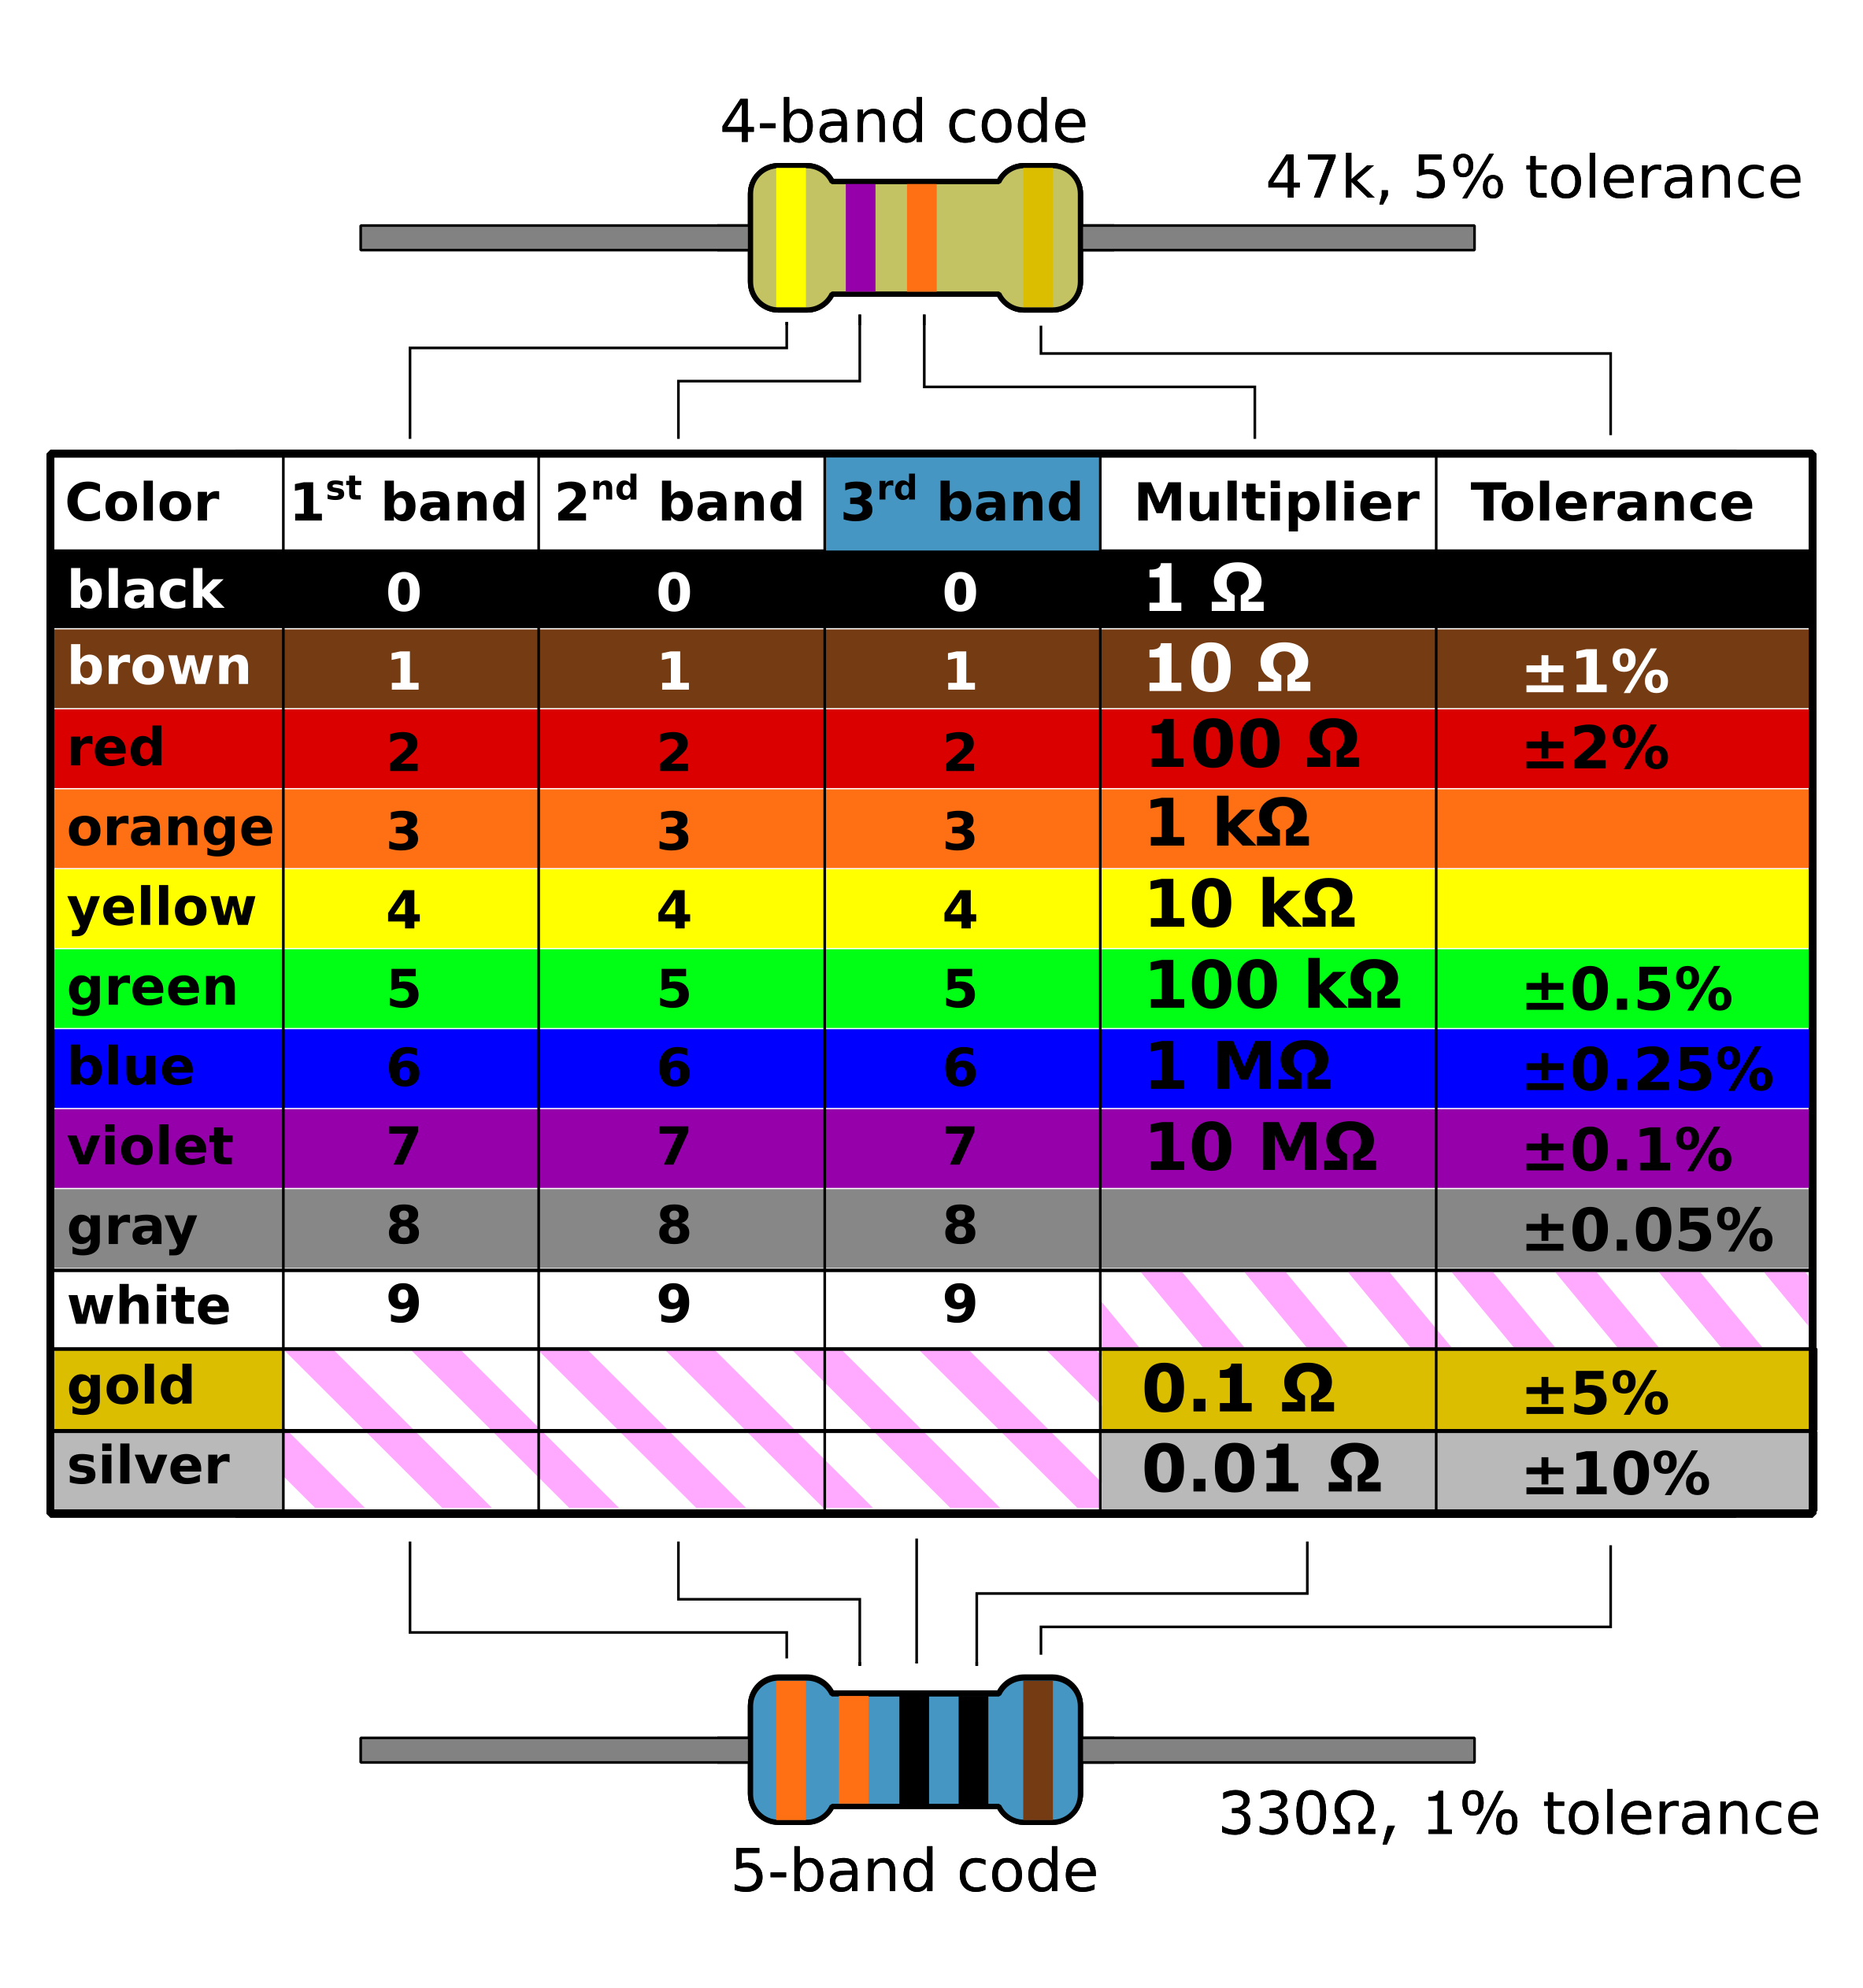
\includegraphics[scale=0.60]{resistorchart.png}
}
\end{center}
\caption{A resistor value color band chart. The `tolerance' stripe (how close the value is guaranteed to be to the stated value) is on the right side. }
\label{fig:resistorchart}
\end{figure}
